\chapter{Tests}
\label{TEST}
\section{White box: closestEdge}
\label{TEST-CE}
A white box test is a test that is made with knowledge of the internal structure
of the code, and uses this knowledge to make sure all flows through the 
code is covered. We are using the ``\class{getClosestNode}'' method for this
test since it contains both loops and conditional statements. The method is supposed
to find the closest \class{Node} to a given point. It accomplishes this by first
searching another method for the closest \class{Edge} (which is trivial). This
procedure is performed with greater and greater search radius until it finds something.
When it has found an \class{Edge}, it will determine which end (\class{Node}) is
closest to the point. In order to secure full coverage of the tests we have created the
following scheme of tests and expected results (using our test graph seen on
page \pageref{TEST-JU-MT-TG}).

\begin{centering}
\begin{tabular}{|p{1.7cm}|p{3cm}|p{3cm}|p{3cm}|}
\hline
\textbf{Part} & \textbf{Case} & \textbf{Input} & \textbf{Expected Output} \\
\hline
\hline
while(once) & Some point that finds an \class{Edge} within the initial search
radius & 6000, 2000, Evaluator.CAR & \class{Node} with index 2\\
\hline
while(more) & Some point that has to widen the search radius in order to find
anything & -200, -200, Evaluator.CAR & \class{Node} with index 4\\
\hline
if-block & The first \class{Node} is closest & 10000, 8500, Evaluator.CAR &
\class{Node} with index 8\\
\hline
else-block & The second \class{Node} is closest & 8500, 8500, Evaluator.CAR
& \class{Node} with index 7\\
\hline
\end{tabular}
\end{centering}

This procedure is great for testing every corner of the code because we are
making a test for reaching all sections within if-statements and make sure we
run while-loops zero, once and multiple times\footnote{We cannot run this while
loop zero times since the loop runs when edge == null and the edge variable is
defined as null just before the loop.}. It should be noted that the white box
tests should be accompanied by black box tests, because these tests uses the
input needed for reaching a specific block. This means they do not check if
invalid input breaks the program. Since some of the input overlaps with what is
needed for the black box, tests they have been located in the same method in our
Model Tests found in appendix \ref{APP-TE-JU-MO} on page
\pageref{APP-TE-JU-MO}\footnote{In the testGetClosestNode() method, the first,
third, fourth and fifth asserts.}.

\section{JUnit}
\label{TEST-JU}
This section describes the JUnit tests we have made for our software. We have
made tests for the public methods in \class{Model}, \class{PointMethods} and
\class{RectangleMethods}.

\subsection{ModelTest}
\label{TEST-JU-MT}
The model class has some of the most interesting functions and algorithms of
our program. The most advanced functions in the model are those regarding path
finding. The task of finding a path from one node of the graph to another,
takes many different kinds of input. The coverage table for the JUnit tests of
the \class{Model} class can be found in appendix \ref{APP-TE-JU-MO} on page
\pageref{APP-TE-JU-MO}.

The tests are chosen so that they test for different input. But they are also
chosen so that they test the logical problems our path finding algorithm might
run into. In order to test these problems properly, we constructed some simple
test data that we knew we could rely on:

\begin{figure}[!ht]
\centering
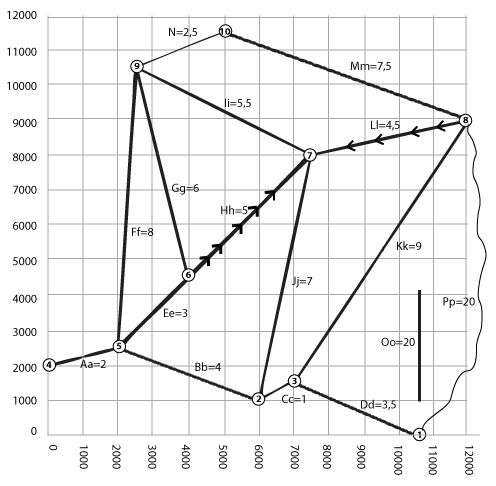
\includegraphics[width=0.6\linewidth]{images/TestGraph}
\caption{Test graph}
\label{TEST-JU-MT-TG}
\end{figure}

Figure \ref{TEST-JU-MT-TG} on page \pageref{TEST-JU-MT-TG} is a visualization
of the graph that we use in our tests. The graph is constructed so that we can
test different problems that might occur in the graph our map uses.

\subsection{PointMethodsTest}
\label{TEST-JU-PMT}
We have tested the public methods in \class{PointMethods} using JUnit testing.
The complete coverage table can be found in appendix \ref{APP-TE-JU-PM} on page
\pageref{APP-TE-JU-PM}.

\subsection{RectangleMethodsTest}
\label{TEST-JU-RMT}
As with the \class{PointMethods} and \class{Model} classes, we have created
JUnit tests for the public methods in \class{RectangleMethods}. We considered
doing more comprehensive testing of the ``newBounds'', ``fixByInnerBounds'' and
``fixByOuterBounds'', but since there are no checks for \class{null} or other
types of bad input for these methods, we felt it was unnecessary. The coverage
table can be found in appendix \ref{APP-TE-JU-PM} on page
\pageref{APP-TE-JU-PM}.

\section{System test}
\label{TEST-ST}
We have written a number of system tests that need to be performed by a
user interacting with the program. These test the basic functionality of the
program as well as some advanced combinations of features. The system tests are
a necessary addition to the unit tests since many bugs are located in the
interactions between algorithms and the user interface, and thus can often not
be found through unit tests. 

The tests have been divided into six groups that increase in
complexity and the later tests may rely on success in previous tests. There are
a total of 34 tests and the complete list and coverage table with instructions
and expected results can be found in appendix \ref{APP-TE-ST} on page
\pageref{APP-TE-ST}. All the tests in the coverage table have been done on a
computer with the Windows 7 operating system.